\chapter{Background}\label{C:backgroundsurvey}
\section{Core Concepts}
\subsection{CNF \& DNF}
A boolean formula is in Conjunctive Normal Form (CNF) if and only if it is a conjunction (and) of clauses. A clause in a CNF formula is given by a disjunction (or ) of literals. A literal is either an atom or the negation of an atom, an atom is one of the variables in the formula.\\

Consider the boolean formula $\lnot a \lor (b \land c)$, the CNF is $(\lnot a \lor b) \land (\lnot a \lor c)$. In this CNF formula the clauses are $(\lnot a \lor b)$, $(\lnot a \lor c)$, the literals used are $\lnot a$, $b$, $c$ and the atoms are $a$, $b$, $c$.\\

A boolean formula is in Disjunctive Normal Form (DNF) if and only if it is a disjunction (or) of clauses. A DNF clause is a conjunction (and) of literals. Literals and atoms are defined the same as in CNF formulas.\\

Consider the boolean formula $\lnot a \land (b \lor c)$, the DNF is $(\lnot a \land b) \lor (\lnot a \land c)$.\\

\subsection{CNF \& DNF from Truth Table}
Given a truth table representing a boolean formula, constructing a DNF formula involves taking all rows which correspond to True and combining them with an OR operation. To construct a CNF one combines the negation of any row which corresponds to False by an OR operation and negates it.

\begin{theorem}
	The maximum number of clauses in a CNF or DNF formula is $2^n$
	\label{thm:max-clause-cnfdnf}
\end{theorem}

\begin{proof}
	Assume the goal is to find the CNF and DNF for a Boolean formula B of size $n$, for which the complete truth table is given. The truth table has exactly $2^n$ rows.\\
	
	First assume a CNF is being constructed, this is achieved by taking the OR of the negation of all rows corresponding to False, the NOT operation leaves the number of clauses unchanged. At most there can be $2^n$ rows corresponding to False, consequently there are at most $2^n$ clauses in the CNF.\\
	
	A similar argument shows that the same holds for DNF.
\end{proof}

\section{Literature Review}

A survey in 1995 focuses on rule extraction algorithms \cite{andrews1995survey}, identifying the reasons for needing these algorithms along with introducing ways to categorise and compare them. Motivation behind scientific study is always crucial so why is understanding the knowledge contained inside Artificial Neural Networks's (ANN's) important? The key points identified are that the ANN might of discovered some rule or patten in the data which is currently not known, being able to extract these rules would give humans a greater understanding of the problem. Another, perhaps more significant reason is the application of ANN's to systems which can effect the safety of human lives, i.e. Aeroplanes, Cars. If using an ANN in the context of a system involving human safety it is important to be certain of the knowledge inside the ANN, to ensure that the ANN wont take any dangerous actions.\\

There are three categories that rule extraction algorithms fall into \cite{andrews1995survey}. An algorithm in the \textbf{decompositional} category focuses on extracting rules from each hidden/output unit. If an algorithm is in the \textbf{pedagogical} category then rule extraction is thought of as a learning process, the ANN is treated as a black box and the algorithm learns a relationship between the input and output vectors. The third category, \textbf{electic}, is a combination of decompositional and pedagogical. Electic accounts for algorithms which inspect the hidden/output neurons individually but extracts rules which represent the ANN globally \cite{tickle1998truth}.\\

To further divide the categories two more classifications are introduced. One measures the portability of rule extraction techniques, i.e. how easily can they be applied to different types of ANN's. The second is criteria to assess the quality of the extracted rules, these are accuracy, fidelity, consistency, comprehensibility \cite{andrews1995survey}.

\begin{enumerate}
\item A rule set is \textbf{Accurate} if it can generalize, i.e. classify previously unseen examples.
\item The behaviour of a rule set with a high \textbf{fedelity} is close to that of the ANN it was extracted from.
\item A rule set is \textbf{consistent} if when trained under different conditions it generates rules which assign the same classifications to unseen examples.
\item The measure of \textbf{comprehensibility} is defined by the number of rules in the set and the number of literals per rule.
\end{enumerate}

In 1996 a class of networks, called Logical Normal Form Networks (LNFNs), where developed \cite{herrmann1996backpropagation}, focusing on learning the underlying CNF or DNF for a boolean expression which describes the problem. The approach relies on a specific network configuration along with restriction the function space of each neuron, allowing them to only perform an OR or AND on a subset of their inputs, such OR and AND neurons are called Disjunctive and Conjunctive retrospectively. If the trained network is able to achieve a low enough accuracy then rules can be extracted from the network in terms of a Boolean CNF or DNF expression \cite{herrmann1996backpropagation}.\\

The algorithm which extracts rules from LNFNs would be Electic and certainly is not Portable as the algorithm is specific to the LNFN architecture. It is not possible to further classify the rule extraction algorithm as the research developing it lacks any experimental results, much justification is also missing making the LNFNs difficult to reproduce.\\

In 2016 the concept of Noisy-OR and Noisy-AND neurons where described \cite{LearningLogicalActivations}, networks containing such Noisy neurons are called Logical Neural Networks (LNNs). Pure LNNs contain only Noisy neurons. This report aims to re derive LNFNs as a subset of Pure LNNs, that is using only Noisy neurons.\\

Noisy neurons are derived from the Noisy-OR relation\cite{LearningLogicalActivations}, developed by Judea Pearl \cite{russell1995modern}, a concept in Bayesian Networks. A Bayesian Network represents the conditional dependencies between random variables in the form of a directed acyclic graph.

\begin{figure}[H]
  \centering
  \begin{minipage}[b]{0.4\textwidth}
    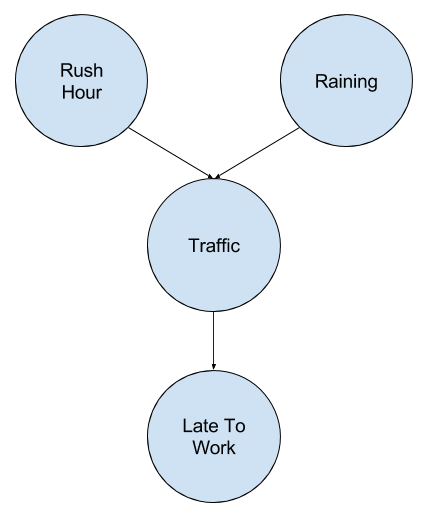
\includegraphics[width=\textwidth]{bayesian-network-example.png}
    \caption{}
    \label{fig:bayesian-network-example}
  \end{minipage}
  \hfill
\end{figure}

Figure \ref{fig:bayesian-network-example} is a Bayesian network, it demonstrates the dependency between random variables "Rush Hour", "Raining", "Traffic", "Late To Work". The connections show dependencies i.e. Traffic influences whether you are late to work, and it being rush hour or raining influences whether there is traffic.\\

Consider a Bayesian Network having the following configuration, take some node $D$ with $S_1,..., S_n$ as parents i.e. $S_i$ influences the node $D$, each $S_i$ is independent from all others. The relationship between D and its parents is if $S_1\ OR\ ...\ OR\ S_n$ is true then $D$ is true. Let $\epsilon_i$ be the uncertainty that $S_i$ influence $D$ then $P(D = 1| S_1 = 1, , S_n = 1)$ can be defined.

\begin{align}
P(D = 1 | S_1 = 1, ..., S_n = 1) = 1 - \prod^n_{i=1} \epsilon_i
\label{equ:noisy-or-relation}
\end{align}

Equation \ref{equ:noisy-or-relation} shows the noisy or relation \cite{LearningLogicalActivations}. In the context of a neuron, the inputs $x_1, ..., x_n$ represent the probability that inputs $1, ..., n$ are true. Consider the output of a neuron as conditionally dependent on the inputs, in terms of a Bayesian Network each $x_i$ is a parent of the neuron. Each $\epsilon_i$ is the uncertainty as to whether $x_i$ influences the output of the neuron. How can weights and inputs be combined to create a final activation value for the neuron. First consider a function $f(\epsilon, x)$ which computes the irrelevance of input x. Some conditions that can be placed on $f$ are given in \cite{LearningLogicalActivations}. (1) $\epsilon = 1$ means that $f(\epsilon, x) = 1$, (2) $x = 1$ means that $f(\epsilon, x) = 1$, (3) Monotonically increasing in $\epsilon$ and decreasing in x. Let $f(x, \epsilon) = \epsilon^x$. The definitions for Noisy-OR and Noisy-AND gates can now be given.

\begin{definition}
A \textbf{Noisy-OR} Neuron has weights $\epsilon_1, ..., \epsilon_n \in (0,1]$ which represent the irrelevance of corresponding inputs $x_1, ..., x_n \in [0,1]$. The activation of a Noisy-OR Neurons is.

\begin{align}
a = 1 - \prod^p_{i=1} (\epsilon_i^{x_i}) \cdot \epsilon_b
\label{equ:noisy-or-activation-1}
\end{align}
\end{definition}

\begin{definition}
A \textbf{Noisy-AND} Neuron has weights $\epsilon_1, ..., \epsilon_n \in (0, 1]$ which represent the irrelevance of corresponding inputs $x_1, ..., x_n \in [0,1]$. The activation of a Noisy-AND Neurons is.

\begin{align}
a = \prod^p_{i=1} (\epsilon_i^{1 - x_i}) \cdot \epsilon_b
\label{equ:noisy-and-activation-1}
\end{align}
\end{definition}

Both these parametrisations reduce to discrete logic gates when there is no noise, i.e. $\epsilon_i = 0$ for all $i$.\\

ANN's containing of Noisy-OR and Noisy-AND neurons are called Logical Neural Networks (LNN's), if the network consists of only Noisy neurons then it a pure LNN. LNN's have been applied to the MINST dataset with promising results. Experiments with different combinations of logical and standard (sigmoid, soft-max) neurons have shown that pure LNN's where able to achieve an error of 8.67\%, where a standard perceptron/softmax network was able to achieve an error of 3.13\%. This reduction in performance does not come without reward, the pure LNN yields a simpler (sparser) and more interpretable network \cite{LearningLogicalActivations}. Training LNN's which are not pure have been shown to have reduced performance (compared to standard ANN's) and no interpretability benefit.\\

% Do we need this part in the final report %
While the concept given in \cite{herrmann1996backpropagation} is the foundation for the work given in this report, the approach presented is different that what has been done. A simpler parametrisation for disjunctive and conjunctive neurons is used, along with better justification and more investigation of the capabilities of LNFN's.
%%%%%%%%%%%%%%%%%%%%%%%%%%%%%%%%%%%%%%%%%%%%%%


LNFNs are based off the idea of learning an underlying boolean formula, what happens when learning problems which consist of continous features? One option is to simply train the networks using the continuous features, the other is to descretise any continuous value.\\

% Talk about motivations for descrete features %

There are a number of categories used to sort various descretization algorithms \cite{liu2002discretization}, three of these categories are defined below.

\begin{enumerate}
	\item \text{Supervised vs. Unsupervised:} Supervised descretization algorithms use class information, as opposed to unsupervised which do not.
	
	\item \text{Dynamic vs. Static:} Dynamic methods descretize features as the classifier is being built. A static algorithm performs all descretization before the lerning begins.
	
	\item \text{Global vs. Local: } Global methods descretize the entire instance space where as local only descretize a subset of the total space.
\end{enumerate}

The types of descretization algorithms which will be considered are Static and Global. Dynamic does not make a lot of sense when the data is used in training an ANN and a Local does not make sense if we are using a Static method. As for Supervised vs. Unsupervised it does not matter, though since we do have access to the labels using them could provide better performance.\\

Basic descretizing methods are \text{Equal width and frequency binning}, these are unsupervised algorithms. Equal width divides the interval up into $K$ equally sized bins, where as equal frequency divides the interval into $K$ bins where each one has the same number of instances. While implementation is easy it is not without a cost, namely results could be poor if the distribution of features is not uniform \cite{liu2002discretization}. The two methods also require that $K$ be pre defined, this could require an expensive trial and error process. \cite{liu2002discretization}.\\

A supervised technique is called \text{Recursive Minimal Entropy Partitioning} (RMEP). Let $S = \{s_1, ..., s_n\}$ be a set of instances, each with $n$ attributes. The goal of RMEP is to partition the range of each attribute. The entropy of a set is given by equation \ref{equ:entropy}

\begin{align}
	E(S) = \sum_{i} p_i \cdot log(p_i)
	\label{equ:entropy}
\end{align}

